
\subsection{Lato Client}

\textcolor{red}{COSE CHE MANCANO A FREPPO: AGGIUNGERE INTERAZIONI CON ANGULAR E D3, MA PER QUELLO SERVER CARDIN. PER IL RESTO CI SIAMO... almeno della mia parte :---------------)}

\begin{figure}[H]
    \centering
    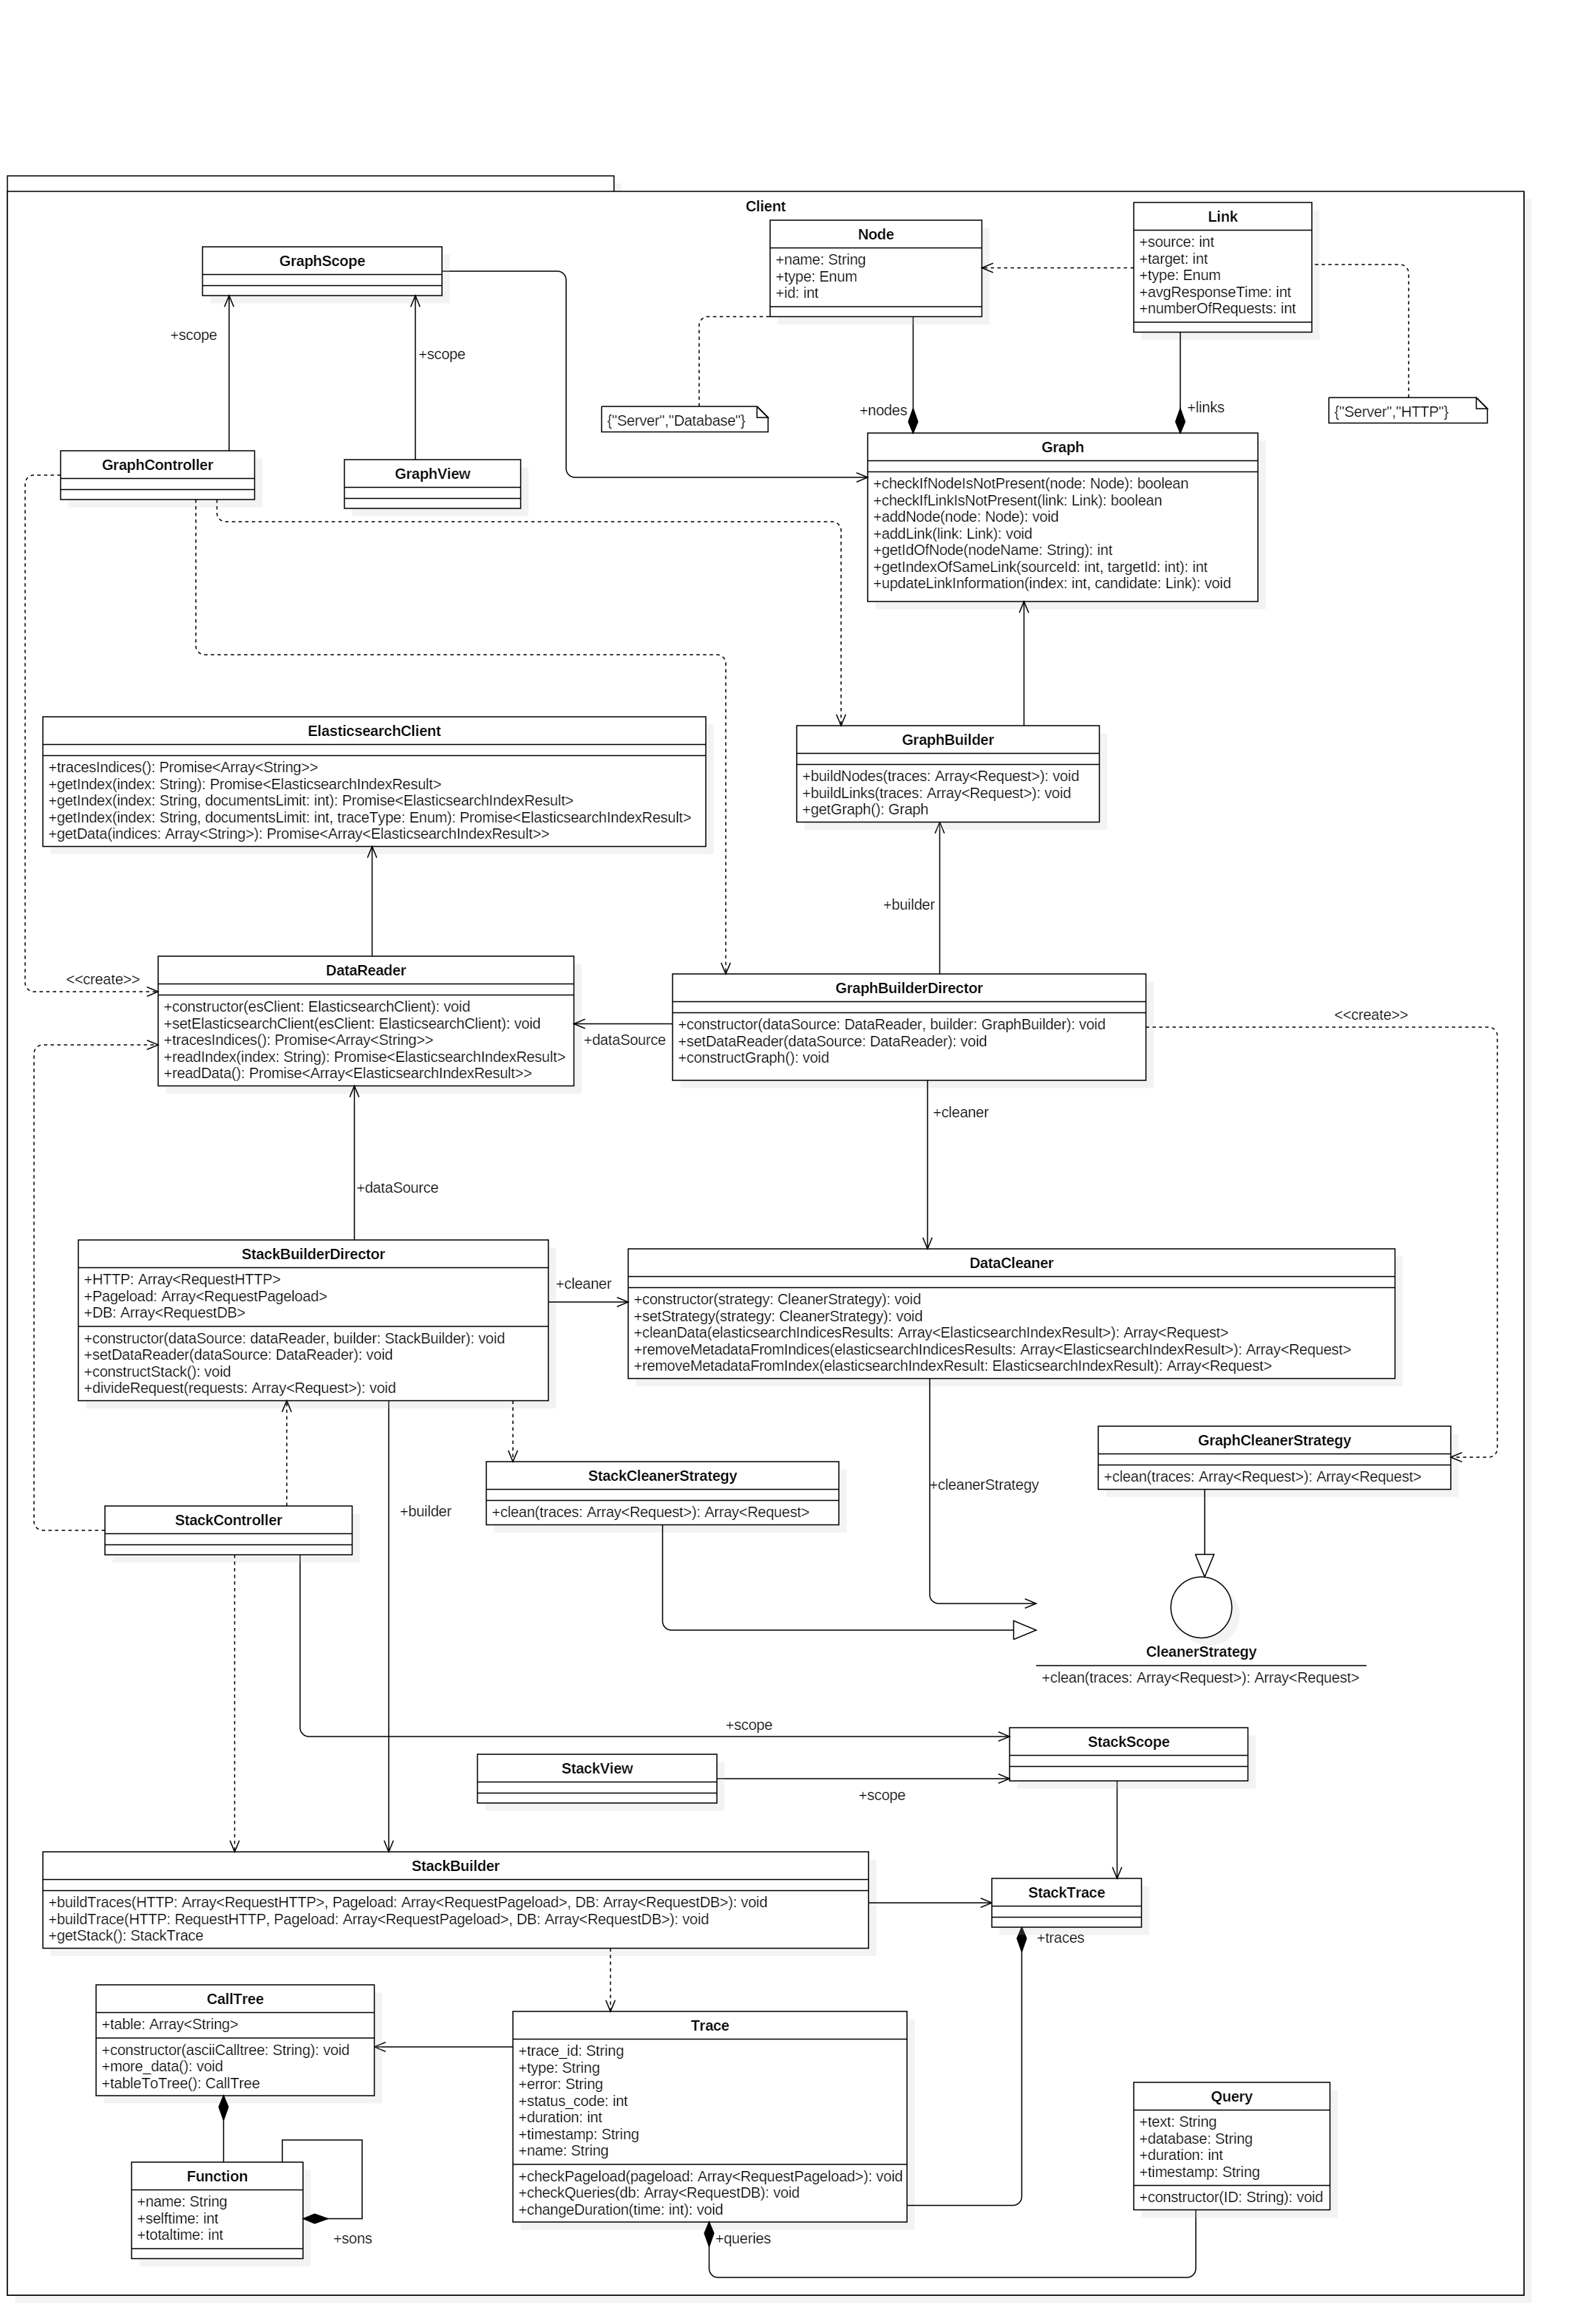
\includegraphics[width=1\textwidth]{Images/classi.png}
    \caption{Diagramma delle classi client-side dell'applicazione}
    \label{img:diagrammaClassiClient}
\end{figure}

\subsubsection{Generalità}
Il lato client si occupa di interrogare il lato server per ottenere informazioni grezze, elaborarle per renderle utili ed infine presentarle all'utente. \texttt{DataReader} si occupa di fornire ai client dati letti dal database Elasticsearch, mentre \texttt{DataCleaner} rimuove da i dati grezzi di tipo \texttt{ElasticsearchIndexResult} le informazioni amministrative, lasciando solamente i documenti veri e propri. Essi vengono elaborati da una coppia di \texttt{Builder} per creare dati che abbiano una interfaccia idonea ad essere mostrata all'utente finale. I dati costruiti sono di tipo \texttt{Graph} per la mappa topologica e di tipo \texttt{StackTrace} per la stack trace. I dati del grafo vengono mostrati all'interno di un \emph{canvas} tramite la libreria grafica D3.js, mentre i dati della stack trace vengono mostrati da Angular, in un template HTML. 

\subsubsection{Componenti} 
\label{sec:Componenti}
Si descrivono di seugito brevemente i componenti del lato client.

\paragraph{ElasticsearchClient} \Spazio
\texttt{ElasticsearchClient} è il componente che si occupa di eseguire le chiamate API al lato server. Non è una classe vera e propria all'interno del codice, ma un \emph{Service}. 
I Service sono funzioni, od oggetti, che possono essere passati a tutte le altri componenti di angularJs attraverso \emph{Dependency Injection}, permettono di condividere codice e funzionalità facilmente. Essi sono \emph{lazily instantiated}, cioè generati solo quando un componente esprime una dipendenza verso un determinato service. Permettono la realizzazione di servizi come i client API, dove avere piú istanze dello stesso client non sarebbe ragionevole. 
Utilizzare un service è l'unico modo per poter eseguire chiamate REST parametrizzate al lato server. Ciascun metodo qui presentato nasconde in realtà una chiamata GET all'opportuno componente lato server. I metodi da esso esposti sono: 
\begin{itemize} 
  \item \texttt{tracesIndices(): Array<String>} ritorna un array di stringhe che rappresenta gli indici contenuti nell'istanza di ElasticSearch che hanno all'interno delle traces, ovvero i dati utili al plugin; 
  \item \texttt{getIndex(index:String): ElasticsearchIndexResult} ritorna al chiamante i dati grezzi che vengono restituiti da Elasticsearch eseguendo una ricerca priva di parametri sull'indice passato come parametro, ovvero \texttt{index}. Essi comprendono, oltre tutti i documenti dell'indice, anche i metadati di Elasticsearch dato che sono di tipo \texttt{ElasticsearchIndexResult}. È anche possibile specificare un numero massimo di documenti ritornati al chiamante o una particolare tipologia letta nel database di tipo \texttt{server} o \texttt{database}; 
  \item \texttt{getData(indices:Array<String>): Array<ElasticsearchIndexResult>}: ritorna al chiamante un array di dati grezzi, ognuno dei quali rappresenta il risultato di una ricerca priva di parametri su un indice. Gli indici letti sono quelli ritornati da \texttt{tracesIndices()}, ovvero tutti e soli quelli che contengono traces. 
\end{itemize} 
Osserviamo che anche se in questa rappresentazione questi metodi sono all'interno di un oggetto, non avendo i diagrammi delle classi UML un costrutto per rappresentare precisamente un \emph{Service}, essi non hanno una struttura ben definita e oggetti di tipo \texttt{ElasticsearchClient} chiaramente non sono istanziabili direttamente dal client. Dunque, per interfacciarsi ad Elasticsearch si è deciso di racchiudere tutte queste funzionalità in un oggetto vero e proprio, \texttt{DataReader} (descritto nella sezione \ref{sec:DataReader}), per poter avere una più agevole interazione con i dati. 

\paragraph{DataReader} \Spazio
\label{sec:DataReader}
\texttt{DataReader} è il componente del sistema che si occupa di reperire i dati da Elasticsearch, ciò viene fatto utilizzando il \emph{Service} \texttt{ElasticsearchClient}. Sarebbe effettivamente possibile utilizzare le chiamate al \emph{Service} ogni qualvolta fossero necessari dei dati, tuttavia ricordiamo che tali chiamate non vengono racchiuse all'interno di un oggetto ben strutturato. DataReader restituirà ai richiedenti le informazioni grezze i tipo \texttt{ElasticsearchIndexResult}, esattamente come vengono restituite da Elasticsearch. I metodi sono:  

\begin{itemize} 
	\item \texttt{constructor(esClient:ElasticsearchClient): void} che costruisce il \texttt{DataReader} parametrizzato con un \texttt{ElasticsearchClient};
	\item \texttt{setElasticsearchClient(esClient:ElasticsearchClient): void}: permette di impostare una sorgente dei dati;
	\item \texttt{tracesIndices(): Array<String>}: ritorna un array di stringhe, i quali elementi sono tutti e soli gli indici all'interno dell'istanza di Elasticsearch che hanno al loro interno delle traces;
	\item \texttt{readIndex(index:String): ElasticsearchIndexResult}: ritorna al chiamante i dati grezzi che vengono restituiti da Elasticsearch eseguendo una ricerca priva di parametri sull'indice passato come parametro, ovvero \texttt{index}. Essi comprendono oltre tutti i documenti dell'indice anche i dati amministrativi di Elasticsearch;
	\item \texttt{readData(): Array<ElasticsearchIndexResult>}: ritorna al chiamante un array di dati grezzi, ognuno dei quali rappresenta il risultato di una ricerca priva di parametri su un indice. Gli indici letti sono quelli contententi delle traces, ovvero quelli utili al plugin. Ciò è realizzato leggendo tali indici grazie al metodo \texttt{tracesIndices()}.
\end{itemize}



\paragraph{DataCleaner}\Spazio
\label{sec:DataCleaner}
\texttt{DataCleaner} è il componente del sistema che si occupa di pulire i dati grezzi che sono stati reperiti da Elasticsearch. Esso compie questo lavoro in due momenti: prima estraendo i dati utili (ovvero i documenti veri e propri) da Elasticsearch e poi pulendoli attraverso una \emph{strategy}, descritta in \ref{sec:CleanerStrategy}.\\
I suoi metodi sono:

\begin{itemize} 
	\item  \texttt{constructor(strategy:CleanerStrategy): void} costruisce il \texttt{DataCleaner} con una specifica strategia di pulizia;
	\item \texttt{setStrategy(in strategy:CleanerStrategy): void} il quale riceve in input un oggetto che implementa l'interfaccia \texttt{CleanerStrategy} e lo assegna al riferimento proprio dell'oggetto;

	\item \texttt{cleanData(in elasticsearchIndicesResults:Array<ElasticsearchIndexResult>): Array<Request>} il quale prima rimuove i metadati (chiamando il suo metodo \\ \texttt{ removeMetaDataFromIndices }) di Elasticsearch dal parametro in input e successivamente chiama l'implementazione di \texttt{clean} della strategia che possiede al suo interno.  Tale strategia è incaricata di raffinare ulteriormente i dati per la costruzione della Mappa Topologica oppure per la costruzione dello Stack Trace tramite il metodo \texttt{clean};

	\item \texttt{removeMetadataFromIndices(elasticsearchIndicesResults: \\Array<ElasticsearchIndexResult>): Array<Request>}  si occupa di rimuovere i metadati di Elasticsearch da un Array di indici invocando il metodo \texttt{removeMetaDataFromIndex} su ognuno dei singoli indici. Viene ritornato un array di \texttt{Request} che rappresenta le traces lette dai vari indici in un singolo array;

	\item \texttt{removeMetadataFromIndex(elasticsearchIndexResult:ElasticsearchIndexResult): Array<Request>} il quale si occupa di rimuovere i metadati di Elasticsearch che sono presenti in un \emph{singolo} indice. Questo metodo ritorna un array contenente i documenti JSON così come essi sono stati inseriti dall'applicazione di monitoring negli indici di Elasticsearch. Elasticsearch, infatti, immagazzina i documenti JSON nel campo \texttt{\_source} il quale è inserito in oggetti che contengono altri dati ed informazioni amministrative. Il metodo si occupa di rimuovere questi dati e restituire un array contenente i documenti di un indice;
\end{itemize}

Risulta chiaro che esiste dunque una dipendenza fra la struttura dei dati che vengono restituiti da ElasticSearch, la classe \texttt{DataCleaner} e le classi che implementano \texttt{CleanerStrategy}. Tuttavia, i client di \texttt{DataCleaner} potranno avere accesso diretto ai dati di ElasticSearch, privi di dati amministrativi.
	
\paragraph{CleanerStrategy}\Spazio
\label{sec:CleanerStrategy}
\texttt{CleanerStrategy} è l'interfaccia che verrà implementata per realizzare una pulizia più raffinata dei dati di un \texttt{DataCleaner}. Espone il metodo \texttt{clean(data)}, che avrà comportamenti diversi a seconda della strategia che si desidera applicare. Dato che il prodotto è implementato in Javascript il costrutto interfaccia non è presente nel linguaggio. Per ovviare a questa mancanza tutte le classi che dovrebbero implementare questa interfaccia \emph{devono} possedere un metodo \texttt{clean(data)} che funzioni come ci si aspetti. Questa interfaccia implementa il design pattern \emph{Strategy}, come descritto in \ref{sec:patternStrategy}.
	
	
\paragraph{GraphCleanerStrategy}\Spazio
\label{sec:GraphCleaner}
\texttt{GraphCleaner} è l'implementazione di \texttt{CleanerStrategy} utilizzata da \texttt{DataCleaner} per pulire i dati che dovranno essere utilizzati per la costruzione del grafo rappresentante la mappa topologica. Esso dispone dei seguenti metodi:
\begin{itemize}
	\item \texttt{clean(traces:Array<Request>): Array<Request>} che riceve come input un Array di indici che contengono al loro interno i documenti JSON sotto forma di Array. Tale metodo agisce scorrendo l'array rimuovendo i documenti inutili alla costruzione del grafo.
\end{itemize}

\paragraph{StackCleanerStrategy} \Spazio
\label{sec:StackCleaner}
\texttt{StackCleaner} è l'implementazione di \texttt{CleanerStrategy} utilizzata da \texttt{DataCleaner} per pulire i dati che dovranno essere utilizzati durante la costruzione della stack trace. Essa dispone del metodo
\begin{itemize}
	\item \texttt{clean(traces:Array<Request>): Array<Request>} il quale scorre tutti i documenti JSON disponibili ed ha come output l'insieme di documenti che rappresentano chiamate HTTP, DB oppure Pageload, ovvero tutte e sole quelle necessarie per la costruzione dei dati strutturati della stack trace.
\end{itemize}



\paragraph{Graph} \Spazio
\label{sec:Graph}
	\texttt{Graph} è il tipo di dato che rappresenta il grafo della mappa topologica dell'applicazione. Esso contiene due Array, uno di \texttt{Nodes} e uno di \texttt{Links}.
	Il tipo di dato \texttt{Graph} contiene i seguenti metodi:
	\begin{itemize}
		\item{\texttt{checkIfNodeIsNotPresent(node:Node): boolean} controlla se l'oggetto che gli viene passato, che è  un \texttt{Node} risulta già essere presente nell'Array \texttt{nodes}; }
		\item{\texttt{checkIfLinkIsNotPresent(link:Link): boolean} controlla se l'oggetto che gli viene passato, che è un \texttt{Link} risulta già essere presente nell'Array \texttt{links}; }
		\item{\texttt{addNode(node:Node): void} aggiunge l'oggetto passatogli, se esso non è già presente;}
		\item{\texttt{addLink(link:Link): void} aggiunge l'oggetto passatogli, se esso non è già presente.}	

		\item{\texttt{getIdOfNode(nodeName:String): int;} scorre l'Array \texttt{Nodes} finchè non trova un \texttt{Node} con campo \texttt{name} uguale a quello passatogli come parametro, ritorna l'\texttt{id} di tale nodo; }
		\item{\texttt{getIndexOfSameLink(sourceId:int, targetId:int): Link} scorre l'Array \texttt{Links} finchè non trova un \texttt{Link} con campi \texttt{source} e \texttt{target} uguali a quelli passati per parametro e in tal caso ritorna tale \texttt{Link};}				
	\end{itemize}

\paragraph{Node} \Spazio
Rappresenta un nodo all'interno dell'applicazione monitorata. Consta dei campi dati: 
\begin{itemize}
	\item \texttt{id}, contiene un id numerico intero univoco che individua un nodo;
	\item \texttt{name}, contiene il nome del nodo. Anche esso è univoco;
	\item \texttt{type}, contiene la tipologia del nodo, che potrà essere \texttt{Server} oppure \texttt{Database}.
\end{itemize}

\paragraph{Link}\Spazio
Rappresenta un collegamento tra due nodi dell'applicazione monitorata. Consta dei campi dati:
\begin{itemize}
	\item{\texttt{source}, che rappresenta il nodo che ha effettuato la chiamata sotto forma di id numerico intero;}
	\item{\texttt{target}, che rappresenta il nodo che ha ricevuto la chiamata sotto forma di id numerico intero;}
	\item{\texttt{type}, che può essere \texttt{Database} o \texttt{HTTP}, per rappresentare i diversi tipi di comunicazione;}
	\item{\texttt{avgResponseTime}, che contiene il tempo medio di risposta di tutte le trace tra source e target;}
	\item{\texttt{numberOfRequests}, che indica quante richieste rappresenta un Link.}
\end{itemize}
Ciascun \texttt{Link} è individuato univocamente dalla coppia di campi dati \texttt{source} e \texttt{target}.

\paragraph{GraphBuilderDirector} \Spazio
È il componente che si occupa di condurre il processo di costruzione di un grafo. Implementa il \emph{pattern} \emph{Builder}, come descritto in \ref{sec:patternBuilder}. Consta dei metodi:
\begin{itemize}
	\item \texttt{constructor(dataSource:DataReader, builder: GraphBuilder): void} che costruisce il \texttt{GraphBuilderDirector} con una sorgente dei dati associata e una istanza di \texttt{GraphBuilder}. Istanzia anche un \texttt{DataCleaner} con strategia \texttt{GraphCleanerStrategy}; 
	\item \texttt{setDataReader(dataSource:DataReader): void} che imposta la sorgente dei dati; 
	\item \texttt{constructGraph(): void}: che si occupa di condurra la costruzioni delle parti dell'oggetto \texttt{Graph} tramite \texttt{GraphBuilder}.
\end{itemize}

\paragraph{GraphBuilder} \Spazio
\label{sec:GraphBuilder}
	\texttt{GraphBuilder} è il componente che si occupa di costruire il grafo di nodi e archi rappresentanti la mappa topologica dell'applicazione, secondo la struttura descritta in \ref{sec:Graph}. Esso verrà successivamente visualizzato utilizzando la libreria D3.js. I metodi della classe sono:
	\begin{itemize}
		\item \texttt{buildNodes(traces:Array<Request>): void} il quale riceve un Array di \texttt{Request} e  costruisce i nodi dell'oggetto \texttt{Graph};
				
		\item\texttt{buildLinks(traces:Array<Request>): void} il quale riceve in input l'Array di \texttt{Nodes} dell'applicazione e un Array di richieste HTTP e a Database e costruisce nell'istanza di \texttt{Graph} i \texttt{Links} . Il metodo scorre tutti i documenti JSON che gli vengono passati come Array e per ogni documento, che contiene la trace di una comunicazione tra due componenti dell'applicazione costruisce un oggetto candidato ad entrare nell'insieme. Il fatto che tale \texttt{Link} candidato non sia già presente nell'insieme viene garantito dal metodo \texttt{checkIfLinkIsNotPresent} che controlla che nell'Array dei links non sia già presente un collegamento con gli stessi campi \texttt{source} e \texttt{target} del candidato; 

		\item{\texttt{getGraph(): Graph} il quale ritorna l'oggetto di tipo \texttt{Graph} costruito.  }
	\end{itemize}

\paragraph{StackTrace} \Spazio
Un oggetto \texttt{StackTrace} rappresenta la lista delle richieste alla applicazione monitorata con una struttura significativa per la futura visualizzazione. Essa contiene un array di oggetti \texttt{Trace}.

\paragraph{Trace} \Spazio
Tramite l'oggetto \texttt{Trace} viene modellata una singola richiesta in maniera tale da ottenere solamente i dati utili alla visualizzazione. Questi dati sono ottenuti dai metodi che implementa:
\begin{itemize}
	\item \texttt{checkPageload(pageload:Array<RequestPageload>): void} il quale, se trova una \texttt{RequestPageload} associata alla \texttt{RequestHTTP} principale, modifica il campo dati \texttt{duration} in base alle due \texttt{Request} ;
	\item \texttt{checkPageload(pageload:Array<RequestPageload>): void} il quale, se trova almeno una \texttt{RequestDB} associata alla \texttt{RequestHTTP} principale, modifica il campo dati \texttt{duration} in base alle \texttt{Request} e implementa il campo dati il campo dati \texttt{queries} ;
	\item \texttt{changeDuration(time:int): void} che viene utilizzato per modificare il campo dati \texttt{duration}.
\end{itemize} 

\paragraph{CallTree} \Spazio
Questo componente rappresenta un albero delle chiamate che vengono scatenate da una richiesta. Si compone dei metodi:
\begin{itemize}
	\item \texttt{constructor(asciiCalltree:String): void} costruttore che assembla un oggetto \texttt{CallTree} a partire da una stringa di caratteri;
	\item more\_data(): void che si occupa della costruzione di una tabella contenente i dati grezzi ricavati dalla stringa ASCII;
	\item \texttt{tableToTree(): CallTree} che costruisce il \texttt{CallTree} a partire dalla tabella creata.
\end{itemize}

\paragraph{Function} \Spazio
Il componente \texttt{Function} rappresenta un metodo che viene eseguito in seguito ad una richiesta all'applicazione monitorata. In esso è presente anche il campo \texttt{sons} di tipo \texttt{Function} che racchiude le funzioni richiamate dalla funzione principale.

\paragraph{Query} \Spazio
Questo componente rappresenta una query fatta ad un particolare database durante una richiesta all'applicazione monitorata. Sono presenti i capi dato:
\begin{itemize}
	\item \texttt{text: String},  testo completo della query eseguita;
	\item \texttt{database: String}, nome del database interrogato;
	\item \texttt{duration: int}, durata totale dell'operazione in ms;
	\item \texttt{timestamp: String}, orario e data di inizio operazione.
\end{itemize}
È presente un costruttore, \texttt{constructor( ID:String): void}, che si occupa di istanziazione dell'oggetto \texttt{Query} e del settaggio dei suoi campi dato l'ID di una \texttt{RequestDB}.

\paragraph{StackBuilderDirector} \Spazio
È il componente che si occupa di condurre il processo di costruzione di una stack trace. Implementa il \emph{pattern} \emph{Builder}, come descritto in \ref{sec:patternBuilder}. 
I metodi che sono implementati in esso sono:
\begin{itemize}
	\item \texttt{constructor(dataSource:DataReader, builder: StackBuilder): void} che costruisce il \texttt{StackBuilderDirector} con una sorgente dei dati associata e una istanza di \texttt{StackBuilder}. Istanzia anche un \texttt{DataCleaner} con strategia \texttt{StackCleanerStrategy}; 
	\item \texttt{setDataReader(dataSource:DataReader): void} che imposta la sorgente dei dati; 
	\item \texttt{constructStack(): void}: che si occupa di condurre la costruzione delle parti dell'oggetto \texttt{StackTrace} tramite \texttt{StackBuilder}.
	\item \texttt{divideRequest(requests: Array<Request>): void} che si occupa di suddividere  gli oggetti di tipo \texttt{Request} in base ai sottotipi della classe, costruendo così i campi dati \texttt{HTTP} di tipo \texttt{Array<RequestHTTP>}, \texttt{Pageload} di tipo \texttt{Array<RequestPageload>} e \texttt{DB} di tipo \texttt{Array<RequestDB>}.
\end{itemize}

\paragraph{StackBuilder} \Spazio
Questo componente si occupa della costruzione effettiva di tutte le componenti di una StackTrace. Per fare ciò utilizza i seguenti metodi:
\begin{itemize}
	\item \texttt{buildTraces(HTTP:Array<RequestHTTP>, Pageload:Array<RequestPageload>, DB:Array<RequestDB>): void} che costruisce una \texttt{StackTrace} a partire dai tre array di sottotipi di \texttt{Request};
	\item \texttt{buildTrace(RequestHTTP, Pageload:Array<RequestPageload>, DB:Array<RequestDB>, in index:String): void} che ricevendo un oggetto \texttt{RequestHTTP} e i due array di \texttt{RequestPageload} e \texttt{RequestDB} costruisce un oggetto \texttt{Trace};
	\item \texttt{getStack(): StackTrace} con la quale ritorna il campo dati di tipo \texttt{StackTrace} una volta costruito.
\end{itemize}



% - DESIGN PATTERNS -

\subsubsection{Design patterns}
Si presentano di seguito i \emph{design pattern} implementati nella progettazione del lato client.

\paragraph{Strategy} \Spazio
\label{sec:patternStrategy}
I componenti adibiti alla costruzione di oggetti complessi come \texttt{Graph} e \texttt{StackTrace} necessitano di un array di \texttt{Request}, che rappresentano i dati che dovranno essere elaborati. Le \texttt{Request} lette dal componente \texttt{DataReader} sono quelle presenti all'interno dell'istanza di Elasticsearch e dunque è possibile che alcune di esse non siano necessarie. Ad esempio, per la costruzione di un \texttt{Graph} le \texttt{Request} di tipo \texttt{RequestPageload} non saranno necessarie e dovranno dunque essere eliminate. Si presenta dunque la necessità di avere un componente che in base all'implementazione utilizzata modifichi il comportamento dell'algoritmo utilizzato. Si è scelto quindi di implementare il pattern \emph{Strategy} per la realizzazione di \texttt{CleanerStrategy}, che permette dunque di pulire i dati di Elasticsearch in base alla strategia istanziata. Una rappresentazione della progettazione è riportata in Figura \ref{img:strategy}.

% QUESTA IMMAGINE DEVE RAPPRESENTARE DATACLEANER, CLEANERSTRATEGY E SOTTOCLASSI
\begin{figure}[h]
	\centering
	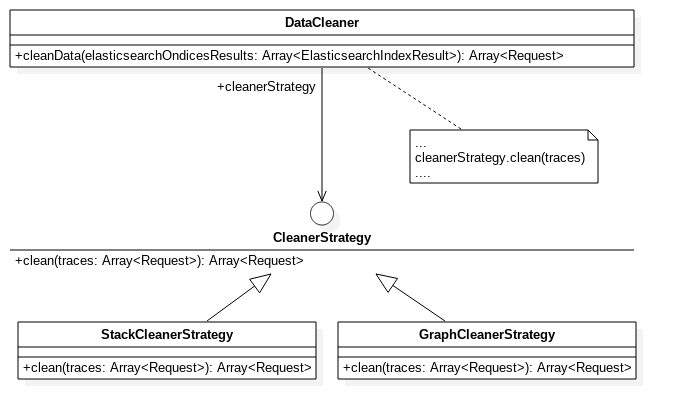
\includegraphics[width=1\textwidth]{Images/patternStrategy.png}
	\caption{Utilizzo del pattern Strategy}
	\label{img:strategy}
\end{figure}
 
\paragraph{Builder} \Spazio
\label{sec:patternBuilder}
I dati rappresentati dal plugin hanno una natura complessa. La mappa topologica deve rappresentare un grafo delle componenti dell'applicazione, mentre la stack trace un array di traces con una forma descritta nella Figura \ref{img:diagrammaClassiClient}. Per tenere separati l'algoritmo di creazione di un oggetto complesso dalle parti di cui lo stesso è composto e dal modo con cui esse sono assemblate si è deciso di applicare in due sezioni differenti il pattern \texttt{Builder}: per la creazione di un \texttt{Graph} e per la creazione di una \texttt{StackTrace}. Le costruzioni di essi sono dirette rispettivamente da un \texttt{GraphBuilderDirector} e un \texttt{StackBuilderDirector}, che ordinano a \texttt{GraphBuilder} e \texttt{StackBuilder} come assemblare le parti. 
Si presenta in Figura \ref{img:builderGraph} il diagramma di sequenza che descrive le interazioni fra i vari componenti che concorrono alla creazione di un oggetto \texttt{Graph}, seguendo il pattern \emph{Builder}.


\begin{figure}[H]
	\centering
	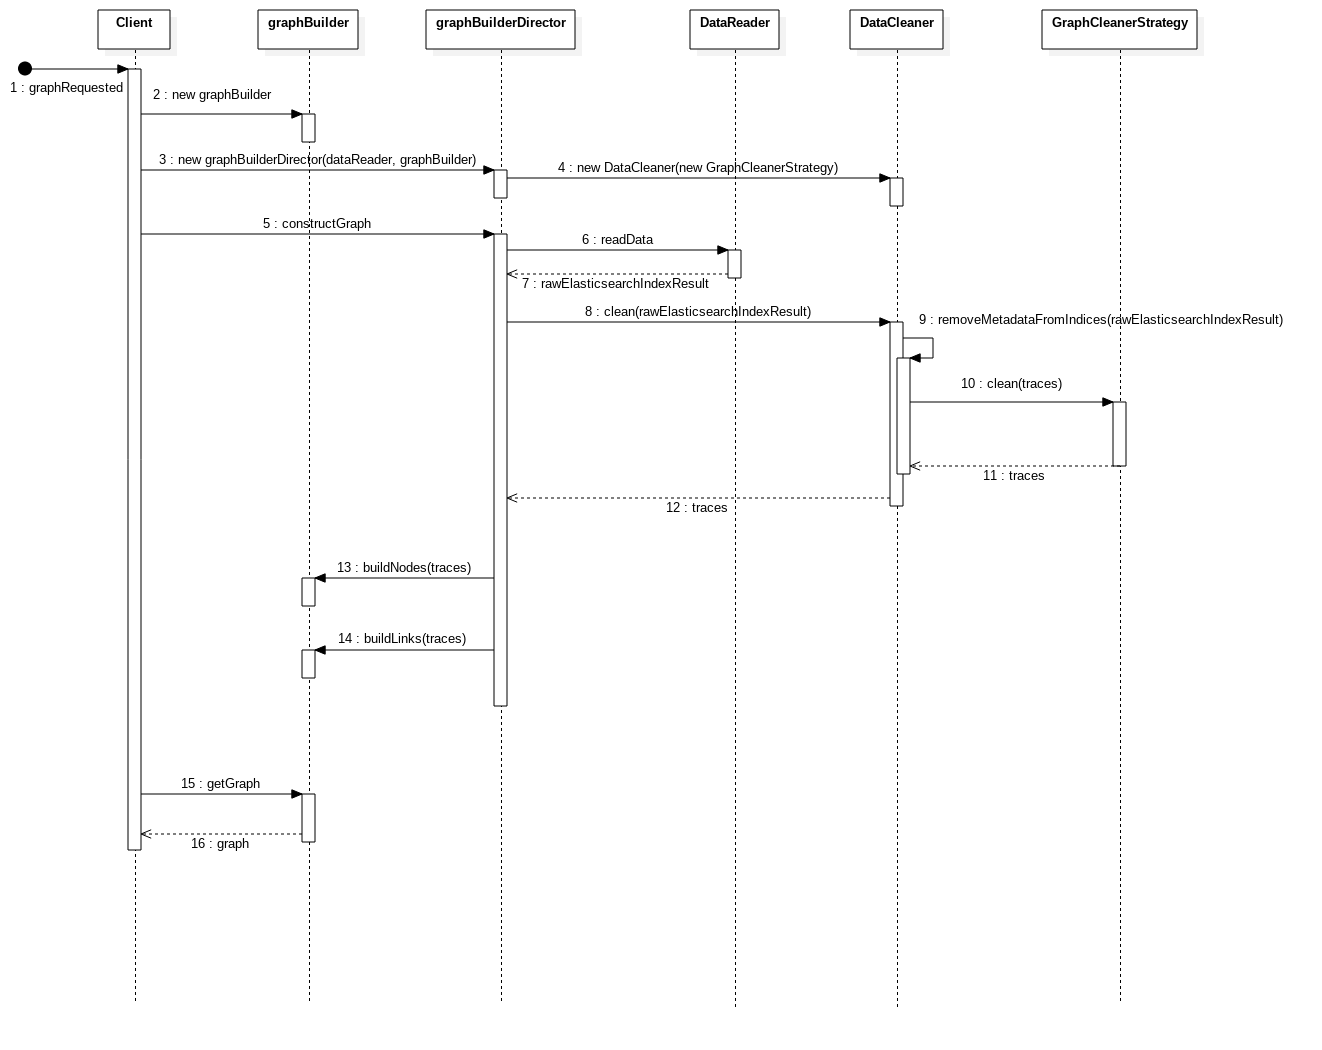
\includegraphics[width=1\textwidth]{Images/builderGraphSequence.png}
	\caption{Diagramma di sequenza che mostra come un client possa ottenere un oggetto \texttt{Graph}}
	\label{img:builderGraph}
\end{figure}

\paragraph{MVVM} \Spazio
\textcolor{red}{QUI CI VA IL MVVM QUANDO SAPRÒ COME RAPPRESENTARLO ALL'INTERNO DI DEL DIAGRAMMA DELLE CLASSI}

\subsubsection{Interazioni}
Si presentano di seguito alcuni diagrammi di sequenza che chiariscono le interazioni fra i vari compoenti del sistema

\paragraph{BuildNodes} \Spazio
Si presenta di seguito il diagramma di sequenza che illustra il comportamento del metodo buildNodes all'interno della classe GraphBuilder.
\begin{figure}[H]
	\centering
	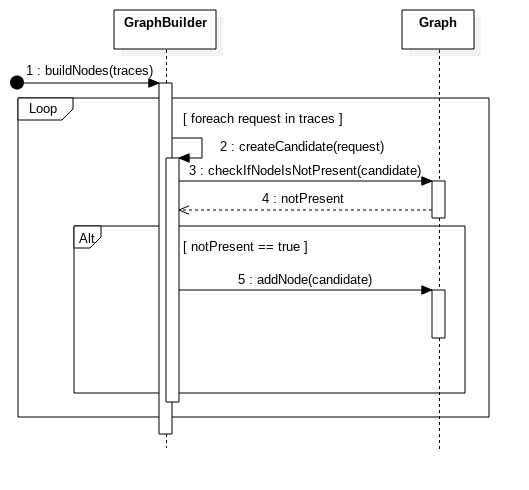
\includegraphics[width=1\textwidth]{Images/SequenceBuildNodes.png}
	\caption{Diagramma di sequenza che illustra il comportamento di \texttt{buildNodes} in GraphBuilder}
	\label{img:sequenceBuildNodes}
\end{figure}

\paragraph{BuildLink} \Spazio
Si presenta di seguito il diagramma di sequenza che illustra il comportamento del metodo buildLinks all'interno della classe GraphBuilder.
\begin{figure}[H]
	\centering
	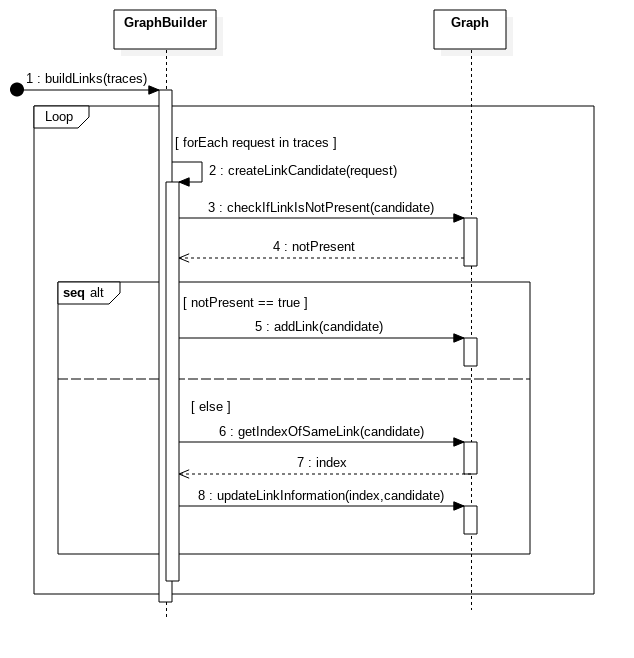
\includegraphics[width=1\textwidth]{Images/SequenceBuildLinks.png}
	\caption{Diagramma di sequenza che illustra il comportamento di \texttt{buildLinks} in GraphBuilder}
	\label{img:sequenceBuildLinks}
\end{figure}

\paragraph{LISA}
\textcolor{red}{LISA METTI QUI I DIAGRAMMI DI SEQUENZA SIGNIFICATIVI PER LA TUA PROGETTAZIONE}
\paragraph{LISA}
\textcolor{red}{LISA METTI QUI I DIAGRAMMI DI SEQUENZA SIGNIFICATIVI PER LA TUA PROGETTAZIONE}












% 	\paragraph{Trace}
% \label{sec:Trace}
% \textcolor{red}{QUI WIPA}
% \texttt{Trace} rappresenta una richiesta che viene fatta al sistema contenente solo i dati veramente utili alla successiva costruzione della Stack Trace. Questi sono:
% \begin{itemize}
% 	\item \texttt{type}: che riconduce ad una delle tipologie di trace;
% 	\item \texttt{trace\_id}: numero univoco che permette l'associazione tra trace HTTP, JDBC e Pageload;
% 	\item \texttt{name}: identificazione generale della richiesta;
% 	\item \texttt{call\_tree}: array contenente gerarchicamente la lista dei metodi invocati dall'applicazione per compiere la richiesta;
% 	\item \texttt{duration}: tempo impiegato dal sistema per lo svolgimento della richiesta, compreso il tempo dei metodi, delle query e del caricamento della pagina;
% 	\item \texttt{timestamp}: data e ora dello svolgimento della richiesta;
% 	\item \texttt{error}: presenza o meno di errori;
% 	\item \texttt{status\_code}: tipologia di errore;
% 	\item \texttt{DBrequest}: (opzionale) array contenente le query con cui è stato interrogato il database.
% \end{itemize}
%  La tipologia delle trace viene identificata tramite i metodi \texttt{checkPageload()} e \texttt{checkQueries()} e queste possono essere:
% 	\begin{itemize}
% 	\item HTTP: insieme di metodi scatenati da un evento generico;
% 	\item HTTP + Pageload: insieme di metodi scatenati dal caricamento di una pagina web;
% 	\item HTTP + JDBC + Pageload: insieme di eventi che portano all'interrogazione di un database e che provocano un successivo caricamento di una pagina.
% 	\end{itemize}
% Inoltre i dati vengono calcolati in base alla tipologia della trace tramite  \texttt{setPageload()} e  \texttt{setQueries()} che utilizzano determinate funzioni per la manipolazione dei dati:
% \begin{itemize}
% 	\item Per il campo \texttt{call\_tree} avviene un'accurata manipolazione attraverso il metodo \texttt{build\_tree()} per passare da un tipo stringa ad una gerarchia di oggetti.
% 	Al metodo \texttt{build\_tree()} viene passato il dato sotto forma di stringa in cui, attraverso l'ASCII art, viene rappresentato un albero dei metodi che vengono invocati con delle informazioni particolari per ognuno di essi. Questo utilizza a sua volta il metodo \texttt{more\_data()} per costruire un array bidimensionale che elenca tutti i metodi e per ognuno ne specifica i dati aggiuntivi rappresentati dall'ASCII art (come total time e self time), il grado di indentazione nell'albero, il numero di metodi figli e il numero di metodi discendenti da esso. \\ Da questa struttura il metodo \texttt{tableToTree()} ricava un oggetto con innestati altri oggetti rappresentanti i metodi e i propri dati strutturati in maniera da rispecchiare i legami di parentela dell'ASCII art.
% 	\item 	Il metodo \texttt{change\_duration} permette di far variare il tempo di esecuzione delle richieste in base alla tipologia in quanto per ognuna bisognerà considerare più parametri per calcolare i millisecondi impiegati.
% \end{itemize}

% \paragraph{StackBuilder}
% \label{sec:StackBuilder}

% \texttt{StackBuilder} si occupa della creazione della struttura della stack trace per la sua successiva visualizzazione.
% Esso viene istanziato con un oggetto \texttt{DataReader} per poter ottenere i dati.
% Il metodo principale è \texttt{getStack()} che controlla tutte le chiamate HTTP ricevute dal \texttt{DataReader} e pulite dal \texttt{DataCleaner}, creato e istanziato con strategia \texttt{StackCleaner}, creando delle \texttt{Trace} da ogni richiesta con dati grezzi.